\documentclass{frontiersSCNS} % for Science articles



\usepackage{graphicx}
%
\usepackage{amsmath} 
\usepackage{mathptmx}      % use Times fonts if available on your TeX system
%
\usepackage{color, soul}
\usepackage{url}
\usepackage{multirow}
\usepackage{array}
\usepackage{fixltx2e}
\usepackage{textcomp}
\usepackage{booktabs}

\usepackage{caption}
\usepackage{subcaption}
\usepackage{float}
\floatstyle{plaintop}

\usepackage{paralist} % inparaenum

\usepackage[bookmarks]{hyperref}

% bibliography
\usepackage[english]{babel}
\usepackage[backend=biber, bibencoding=utf8, style=authoryear, citestyle=authoryear-comp, autocite=inline]{biblatex}
\addbibresource{Bibliography.bib}

\usepackage[draft, nomargin, marginclue, footnote]{fixme}
\fxsetup{targetlayout=color}

% new commands and shortcuts
\usepackage{xspace}
\newcommand{\eg}{\textit{e.g.}\xspace}
\newcommand{\etal}{\textit{et al.}\xspace}
\newcommand{\ie}{\textit{i.e.}\xspace}
\newcommand{\etc}{\textit{etc.}\xspace}
\newcommand{\vs}{\textit{vs.}\xspace}

% shortcut for float placing
\usepackage{placeins}

% make pretty MATLAB code
\usepackage{listings}
\usepackage{matlab-prettifier}
\lstMakeShortInline[style=Matlab-editor]"

\usepackage{xifthen}% provides \isempty test

\copyrightyear{}
\pubyear{}

\def\journal{Neuroinformatics}
\def\DOI{}
\def\articleType{Technology Report}
\def\keyFont{\fontsize{8}{11}\helveticabold }
\def\firstAuthorLast{Hoyland {et~al.}} 
\def\Authors{Alec Hoyland\,$^{1\dagger}$, Srinivas Gorur-Shandilya\,$^{1\dagger}$, and Eve Marder$^{1*}$}
\def\Address{$^{1}$Volen Center for Complex Systems and Biology Department \\ Brandeis University \\ Waltham, MA \\
\vspace{0.25cm}

\vspace{0.5em}\tiny{$\dagger$ These authors have equally contributed to this article.}
}
\def\corrAuthor{Eve Marder \vspace{1mm}}
\def\corrAddress{Marder Lab, Brandeis University, Biology Department and Volen Center for Complex Systems, Waltham, MA, USA}
\def\corrEmail{marder@brandeis.edu}

\begin{document}
\onecolumn
\firstpage{1}

\title[xolotl: neuronal simulator]{Xolotl: An Intuitive and Approachable Neuron \& Network Simulator in MATLAB}
\author[\firstAuthorLast ]{\Authors}
\address{}
\correspondance{}
\extraAuth{}
\topic{An Intuitive Neuronal Simulator}

\maketitle


\begin{abstract}
	
	\texttt{xolotl} is a free and open-source neuronal simulator written in \texttt{C++} with \texttt{MATLAB} wrappers. Biophysically-detailed models of networks can be designed efficiently using an intuitive language tightly coupled to the object-based architecture of the underlying \texttt{C++} code. Models can be specified by adding conductances to compartment objects. The structure is modular, serialized, and searchable, permitting high-level programmatic control over nearly all features of the models. \texttt{C++} templates are provided for developing new conductances, compartments, and integration schemata. It also includes a customizable graphical user interface (GUI) for rapid prototyping and hand-tuning conductances in real-time. The modular structure and accessibility to all parameters, variables, and dynamics of the model network in \texttt{MATLAB} facilitate rapid construction and assessment of model networks. \texttt{xolotl} is freely available at \url{https://github.com/marderlab/xolotl}. This tool provides straightforward implementation and fast simulation of neuronal models while permitting full control over every aspect of the network and integration.
	
	\tiny
	\keyFont{ \section{Keywords:} simulator, MATLAB, C++, conductance-based, neuron, network, keyword} %All article types: you may provide up to 8 keywords; at least 5 are mandatory.
	
\end{abstract}

%%%%%%%%%%%%%%%%%%%%%%%%%%%%%%%%%%%%%%%%%%%%%%%%%%%%%%%%%%%%%%%%%%%%%%%%%
%
%
%
%		INTRODUCTION & OVERVIEW
%
%
%
%%%%%%%%%%%%%%%%%%%%%%%%%%%%%%%%%%%%%%%%%%%%%%%%%%%%%%%%%%%%%%%%%%%%%%%%%


\section{Introduction}
\label{sec:intro}

\texttt{xolotl} (\url{https://github.com/marderlab/xolotl}) is a fast single-compartment and multi-compartment simulator in \texttt{C++} with \texttt{MATLAB} wrappers. Written with an emphasis on ease-of-use, \texttt{xolotl} can simulate single-compartment conductance-based models, networks of these, and detailed multi-compartment models. \texttt{xolotl} exploits a novel automatic type system, \texttt{cpplab}, which binds \texttt{MATLAB} code to \texttt{C++} header files, creating objects and classes \textit{ad libitum} in \texttt{MATLAB} which reflect the underlying object-oriented code. \texttt{xolotl} implements \texttt{cpplab} to represent the nested structure of conductance-based models, and exploits the computational efficiency of the low-level programming language to quickly integrate models. For this reason, models can be implemented entirely in \texttt{MATLAB} with a few lines of code.

Models are specified in \texttt{MATLAB} by a nested structure. The \texttt{xolotl} object contains compartments which themselves contain conductances. Synapses belong to the \texttt{xolotl} object and connect compartments together. The high-level specification supports arbitrarily large network and multi-compartment morphologies. 

%\texttt{xolotl} provides parameter optimization capabilities through the algorithm-agnostic \texttt{procrustes} toolbox. Any network parameters accessible through the \texttt{xolotl} structure can be optimized using arbitrary algorithms and objective functions on multi-core computers and high-performance computing clusters.

The software has been implemented in \texttt{MATLAB} due to its ease-of-use and popularity among neuroscientists. \texttt{cpplab} provides a powerful backend for specifying and integrating models without relying on the significantly slower and limiting \texttt{MATLAB codegen}. While automated \texttt{C++} transpiling from \texttt{MATLAB} using the proprietary \texttt{codegen} can drastically improve performance over loops through strong typing and memory pre-allocation, supervenience of \texttt{MATLAB} over \texttt{C++} prevents efficient use of low-level features, such as passing by reference and object-oriented programming.   Minimal experience with \texttt{MATLAB} is required to use \texttt{xolotl}, and all equations and integration methods are provided transparently to the end user. No string parsing of equations is required \autocite{sherfeyDynaSimMATLABToolbox2018, stimbergBrianSecondComing2013, stimbergEquationorientedSpecificationNeural2014}. 

\texttt{xolotl} comes packaged with visualization functions and a graphical user interface (GUI) for real-time manipulation of model parameters. Plotting of voltage, intracellular calcium, conductance gating functions, and time constants is provided by built-in \texttt{xolotl} methods. The GUI permits real-time tuning of any network parameters using numerical sliders in a graphical interface which displays the resultant membrane potential and intracellular calcium traces. The ease-of-use of these tools lends them to pedagogical applications and rapid exploration of toy models. This tool aims to simplify the investigation of dynamics of complex neural network models, facilitate collaborative modeling, and complement other tools being developed in the neuroinformatics community.

%%%%%%%%%%%%%%%%%%%%%%%%%%%%%%%%%%%%%%%%%%%%%%%%%%%%%%%%%%%%%%%%%%%%%%%%%
%
%
%
%		DESIGN GOALS
%
%
%
%%%%%%%%%%%%%%%%%%%%%%%%%%%%%%%%%%%%%%%%%%%%%%%%%%%%%%%%%%%%%%%%%%%%%%%%%

\section{Design Goals}
\label{design}

"xolotl" is designed to be easy-to-use without sacrificing speed. The software has been designed in "MATLAB" due to its popularity among neuroscientists for pedagogy and research. "xolotl" capitalizes on "MATLAB"'s straightforward structure array syntax to permit rapid prototyping and experimentation, especially for small neuronal networks of complex models. Parameters of conductances, neuronal compartments, and simulations may all be edited in the structure before any calls to integration functions. The underlying code is written in "C++" for speed and memory optimization, and while models can indeed be integrated using the compiled binary, symbolic manipulations can be readily performed in "MATLAB" without ever touching the foundational code. 

\subsection{Features}
\label{features}

Models are specified by adding compartments and synapses to the \texttt{xolotl} object. Conductances are added to compartments and controllers can be added to conductances. This modular structure recapitulates the biophysics of the Hodgkin-Huxley formalism and obviates the need to explicitly write out equations, which in \texttt{xolotl} are contained within the conductance header files.

\texttt{xolotl} relies on \texttt{cpplab} constructions, which allow the user to exploit the efficiency of low-level \texttt{C++} code. \texttt{MATLAB} treats \texttt{cpplab} objects as fully-typed variables allowing for symbolic manipulation using only the high-level programming language and graphical interfaces. \texttt{xolotl} is fast because all time-intensive code is written in \texttt{C++}. While automated \texttt{C++} transpiling from \texttt{MATLAB} using the proprietary \texttt{codegen} can drastically improve performance over loops through strong typing and memory pre-allocation, supervenience of \texttt{MATLAB} over \texttt{C++} prevents efficient use of low-level features, such as passing by reference and object-oriented programming. 

\texttt{C++} provides speed improvements beyond the benefits of translating \texttt{MATLAB} features into low-level code. For this reason, \texttt{cpplab} has been designed to provide an interface for constructing, transpiling, and compiling \texttt{C++} code to be called from within \texttt{MATLAB}. \texttt{xolotl} simulations are run entirely from \texttt{C++} executables. 

\texttt{xolotl} automatically uses the MD5 algorithm to hash the network and compile a new binary and \texttt{MEX} bridge file only if needed. \texttt{MATLAB} provides a high level programmatic and graphical interface for implementing, manipulating, and visualizing models without sacrificing the enhancements of the underlying \texttt{C++} code.

\paragraph{Using the \texttt{cpplab} framework.}

The \texttt{add} function will construct a \texttt{cpplab} object and affix it to as a field in the \texttt{xolotl} structure. All compartments, conductances, synapses, and controllers are \texttt{cpplab}. Compartments add to the \texttt{xolotl} object and conductances add to compartments. Specific properties can be specified using key-value pair arguments (e.g. \ref{fig:figurehh}A).

\texttt{cpplab} comes with several features which simplify the handling of complexly-nested models. The \texttt{find} function acquires a cell array of all properties of the network which satisfy a search condition. For example, one can find all paths to maximal conductances within the "'HH'" compartment by: 

\begin{lstlisting}[style=Matlab-editor]
x.find('HH*gbar');
\end{lstlisting}

To extract a vector of the maximal conductances:

\begin{lstlisting}[style=Matlab-editor]
gbars = x.get(x.find('HH*gbar'));
\end{lstlisting}

To set the maximal conductances all at once:

\begin{lstlisting}[style=Matlab-editor]
x.set('HH*gbar', gbars)
\end{lstlisting}

"MATLAB" can easily control the "cpplab" objects using the standard, flexible data structure notation popular in high-level scripting languages.

\paragraph{Compartments and synapses.}

A model neuron consists of one or more compartments, each representing a section of membrane with capacitance and surface area. Isopotential models require one compartment, whereas models with multiple neurons, units, or non-trivial morphology require multiple compartments. All specifiable properties of compartments are shown in Supplementary Table 1.

\texttt{xolotl} provides some features for generating complex models. Synapses can be added with the \texttt{connect} function. At minimum synapses possess identifiers to presynaptic and postsynaptic compartments and default to electrical synapses. All specifiable properties of synapses are shown in Supplementary Table 2. To create axons or transport chains, the \texttt{slice} function splits a compartment into $n$ discrete segments and adds these compartments to the network connected by electrical synapses.

\paragraph{Conductances and controllers.}

All conductances contain fields for maximal conductance and reversal potential. Conductances with activation and inactivation variables include them as $m$ and $h$ respectively. Gating functions and their respective time constants are contained within the conductance header file. \texttt{xolotl} comes packaged with conductances from several dozen papers (Supplementary Table 3).

\paragraph{Creating custom \texttt{cpplab} objects.}

\texttt{xolotl} contains template header files for producing custom conductances. The template contains instructions on how to design novel conductances with arbitrary specifications.

\paragraph{Simulation.}

Models are simulated in \texttt{xolotl} with the \texttt{integrate} function which outputs as time series the membrane potentials, intracellular calcium concentrations, controller states, intrinsic currents, and synaptic currents. The \texttt{integrate} function also accepts an argument which specifies injected current or clamped voltage. 

"xolotl" uses the exponential Euler method for single compartment models, forward Euler for gating variables, and a Crank-Nicholson regime for electrically-coupled compartments \autocite{ohErrorAnalysisSpecialized2006, dayanTheoreticalNeuroscience2001, butcherNumericalDifferentialEquation2016}. These defaults provide a mix of speed, accuracy, and stability, and are built into the "cpplab" header files. Custom "cpplab" header files can be customized with any iterative integration method. The simulation time-resolution can be specified to target arbitrary precision, and an output time step can be selected to support automatic down-sampling for memory considerations.

Simulations can be run in 'closed-loop' mode where each simulation begins by resetting all dynamical variables to their initial conditions at instantiation, or 'open-loop' mode which begins simulation with the current network state.

\paragraph{Using the graphical interface to manipulate parameters.}

\texttt{xolotl} comes packaged with a graphical user interface for visualizing parameter changes in real-time. The \texttt{manipulate} function opens the GUI, which displays a figure plotting the membrane potential and intracellular calcium concentration of all compartments as time series, and a dialog box with customizable sliders for all parameters of the model, much like the "Manipulate" function in Wolfram "Mathematica". Moving the sliders integrates the model in `open-loop` mode with the new parameters. The parameters available in the sliders can be customized by passing a cell array to manipulate. For example, to only see sliders for maximal conductances of the "HH" compartment, call "x.manipulate(x.find('HH*gbar'))". Closing the GUI saves the network state of the model to the "xolotl" object. This is particularly helpful for rapid prototyping of models.

\paragraph{Optimizing parameters.}
"xolotl" can use the Global Optimization toolbox for "MATLAB" to optimize any accessible "xolotl" parameters. The toolbox is algorithm-agnostic and accepts any function in "MATLAB" with a scalar first output as the objective function. Simulations run on multi-core processors or high-performance computing clusters using the Parallel Computing toolbox.

\subsection{Limitations}
\label{limitations}

The focus on ease-of-use and speed means some features were elided in the streamlining process. 

\paragraph{Reliance on compiled \texttt{C++} code.} While "MATLAB" comes with robust features for compiling "C" and "C++" code, "xolotl" cannot run without "C++" compilation. For users, this necessitates the additional step of setting up the "mex" compiler which can be problematical, especially for nonstandard (e.g. Arch-based Linux). Secondly, compilation adds a small amount to total processing time. Longer simulations ($>1000$ time-steps) minimizes this effect. Adding new conductances also requires writing some "C++" code. For model conductances in the Hodgkin-Huxley formalism \autocite{hodgkinMeasurementCurrentvoltageRelations1952, dayanTheoreticalNeuroscience2001}, adjustments consist of changing default values in a template "C++" header file. Implementing a new integration scheme requires much more in-depth usage of "C++".

\paragraph{Limited to conductance-based models.} "xolotl" has been developed specifically for conductance-based models. It does not currently support current-based models.

\paragraph{Limited numerical integration strategies.} While the exponential Euler method performs well in neuronal models \autocite{ohErrorAnalysisSpecialized2006, dayanTheoreticalNeuroscience2001}, it may be desirable to use other methods under certain conditions. "xolotl" does not currently support other integration schemes for its build-in conductances, nor does the software support error-sensitive variable step-sizes.

\paragraph{Inefficient tools for handling large networks.} While "xolotl" can integrate large networks ($>1000$ compartments), the tools used to index, label, hash, and search large networks become prohibitively slow. "xolotl" uses string-based comprehension for labeling compartments, which is suited to descriptively-named compartments, but computationally slow for searching and indexing.

%%%%%%%%%%%%%%%%%%%%%%%%%%%%%%%%%%%%%%%%%%%%%%%%%%%%%%%%%%%%%%%%%%%%%%%%%
%
%
%
%		USAGE EXAMPLES
%
%
%
%%%%%%%%%%%%%%%%%%%%%%%%%%%%%%%%%%%%%%%%%%%%%%%%%%%%%%%%%%%%%%%%%%%%%%%%%

\section{Usage Examples}
\label{usage}

Using \texttt{xolotl} in \texttt{MATLAB}, users create a \texttt{xolotl} object and populate it with "cpplab" objects which describe compartments, conductances, synapses, and controllers. The model is integrated with the \texttt{integrate} function where the membrane potential, intracellular calcium concentration, controller states, intrinsic currents, and synaptic currents can be outputs.

\texttt{xolotl} comes packaged with a library of pre-existing conductance and synapse objects which greatly simplify the task of constructing model neurons. These objects can be referenced by name and added directly to a compartment. Novel conductance dynamics can be easily written by modifying a template header file contained in the \texttt{xolotl} distribution, or designed entirely from scratch.

%%%%%%%%%%%%%%%%%%%%%%%%%%%%%%%%%%%%%%%%%%%%%%%%%%%%%%%%%%%%%%%%%%%%%%%%%
%
%
%
%		SIMULATING A HODGKIN-HUXLEY MODEL
%
%
%
%%%%%%%%%%%%%%%%%%%%%%%%%%%%%%%%%%%%%%%%%%%%%%%%%%%%%%%%%%%%%%%%%%%%%%%%%

\subsection{Simulating a Hodgkin-Huxley Model}

The seminal Hodgkin-Huxley model of action potentials in the squid giant axon \autocite{hodgkinComponentsMembraneConductance1952, hodgkinMeasurementCurrentvoltageRelations1952} contains a fast inactivating sodium conductance ("NaV"), a non-inactivating delayed rectifier ("Kd"), and a passive leak current (\ref{fig:figurehh}A). A compartment, \texttt{HH}, with membrane capacitance ("Cm") and surface area ("A") can be specified by \ref{fig:figurehh}B. Network properties can be set during construction or afterwards using dot-notation in \texttt{MATLAB} (e.g. \texttt{x.HH.Cm}). \ref{fig:figurehh}C shows the \texttt{MATLAB} command prompt after invoking the \texttt{xolotl} object \texttt{x}, displaying the hierarchical structure inherent in conductance-based treatments of neurodynamics.

This model was constructed using conductances from \cite{liuModelNeuronActivitydependent1998} based on electrophysiological recordings from the lobster stomatogastric ganglion \autocite{turrigianoSelectiveRegulationCurrent1995}. In the absence of applied positive current, the model is quiescent. When 0.2 nA is injected, the model tonically spikes (\ref{fig:figurehh}D). The \texttt{integrate} function takes the applied current as an argument (e.g. "x.integrate(Iapp)"), so that the \texttt{xolotl} object is agnostic to integration-specific perturbations. The \texttt{plot} function generates voltage and intracellular calcium traces, where the voltage trace is colored by the dominant current. If the membrane potential is increasing, the strongest instantaneous inward current colors the trace. Conversely, if the membrane potential is decreasing, the strongest outward current colors the trace instead. \ref{fig:figurehh}F-I display the results of the \texttt{show} function. Activation and inactivation steady-states and the voltage-dependent time constants of these gating variables describe the conductance dynamics in absence of other channel types.

%%%%%%%%%%%%%%%%%%%%%%%%%%%%%%%%%%%%%%%%%%%%%%%%%%%%%%%%%%%%%%%%%%%%%%%%%
%
%
%
%		VOLTAGE CLAMP
%
%
%
%%%%%%%%%%%%%%%%%%%%%%%%%%%%%%%%%%%%%%%%%%%%%%%%%%%%%%%%%%%%%%%%%%%%%%%%%	

\subsection{Performing a Voltage Clamp Experiment \textit{in-silico}}

\texttt{xolotl} can recapitulate the results of voltage clamp experiments \autocite{turrigianoSelectiveRegulationCurrent1995, swensenMultiplePeptidesConverge2000, swensenModulatorsConvergentCellular2001, destexheDynamicClampPrinciplesApplications2009}. Figure \ref{fig:figureclamp} displays steps in the procedure to clamp the membrane potential of a cell with delayed rectifier potassium conductance. During an \textit{in-vitro} experiment, confounding currents would be pharmacologically-blocked and two-electrode voltage clamp used to record tail currents at fixed membrane potential \autocite{connorInwardDelayedOutward1971, connorVoltageClampStudies1971}.

A single-compartment model with a delayed-rectifier conductance is simulated at stepped membrane potentials. The model is simulated using the "integrate" function. The second argument determines the clamped voltage and the fourth output is the current trace.

\begin{lstlisting}[style=Matlab-editor]
	[V, Ca, ~, I] = x.integrate([], clamped_voltage)
\end{lstlisting}

Currents under voltage clamp approach the steady-state holding current (\ref{fig:figureclamp}D-E). The current-voltage relation is the steady-state current over the clamped voltage, and the effective conductance is the derivative of that relation (\ref{fig:figureclamp}F-G). Since the effective conductance is the product of the maximal conductance and the gating variables \autocite{dayanTheoreticalNeuroscience2001, turrigianoSelectiveRegulationCurrent1995} and the tail current is monotonically-increasing with time under voltage clamp, the current can be represented as non-inactivating. Fitting a sigmoid to various powers yields a model for the current dynamics (\ref{fig:figureclamp}H-I). These figures describe graphically the theoretical underpinnings of current analysis through voltage clamp and can serve as an effective pedagogical tool for computational and quantitative neuroscience.

%%%%%%%%%%%%%%%%%%%%%%%%%%%%%%%%%%%%%%%%%%%%%%%%%%%%%%%%%%%%%%%%%%%%%%%%%
%
%
%
%		NETWORK MODELS
%
%
%
%%%%%%%%%%%%%%%%%%%%%%%%%%%%%%%%%%%%%%%%%%%%%%%%%%%%%%%%%%%%%%%%%%%%%%%%%

\subsection{Simulating Network Models}

Network models in \texttt{xolotl} consist of compartment objects connected by synapses. Synapses are stored in a vector array as a field of the \texttt{xolotl} object in \texttt{MATLAB}. Presynaptic and postsynaptic labels indicate the connectivity of the synapse. Figure \ref{fig:figurenetwork} implements a model of the triphasic pyloric rhythm in the stomatogastric ganglion of crustaceans. The pyloric model contains three compartments and seven synapses (\ref{fig:figurenetwork}A). This structure is reciprocated in the hierarchy of the \texttt{xolotl} object, where conductances are contained within compartments (\ref{fig:figurenetwork}B).

Representing the network in "xolotl" requires constructing three compartments and eight conductances in each using the "add" function. 

\begin{lstlisting}[style=Matlab-editor]
	x.add('AB', 'compartment', 'Cm', 10, 'A', 0.628, ...)
	x.AB.add('prinz/NaV', 'gbar', 1000, 'E', 50)
	...
\end{lstlisting}

Synapses are upper-level properties of the network which point between two compartments (\ref{fig:figurenetwork}C). This exploits vectorized operations in \texttt{MATLAB} and does not require each synapse to possess a unique name. The "connect" function adds synapses to the network.

\begin{lstlisting}[style=Matlab-editor]
	x.connect('AB', 'LP', 'Chol', 'gbar', 30)
\end{lstlisting}

%%%%%%%%%%%%%%%%%%%%%%%%%%%%%%%%%%%%%%%%%%%%%%%%%%%%%%%%%%%%%%%%%%%%%%%%%
%
%
%
%		INTEGRAL CONTROL
%
%
%
%%%%%%%%%%%%%%%%%%%%%%%%%%%%%%%%%%%%%%%%%%%%%%%%%%%%%%%%%%%%%%%%%%%%%%%%%

\subsection{Simulating Integral Control}

\texttt{xolotl} can implement homeostatic tuning rules as integral control. The controller computes an error signal (typically a function of intracellular calcium concentration), and adjusts the conductance or synapse it controls accordingly \autocite{olearyCorrelationsIonChannel2013}. In "xolotl", integral controllers are "cpplab" objects added to the conductance or synapse they regulate.

In a demonstration adapted from \cite{olearyCorrelationsIonChannel2013}, integral control changes maximal conductances to bring a neuron from quiescence into a bursting regime. Calcium sensors supervene on maximal conductance density (\ref{fig:figureintegralcontrol}) to change neuronal activity. Each conductance in the "xolotl" structure contains a calcium-sensitive controller (\ref{fig:figureintegralcontrol}B-C). Maximal conductances increase from random initial conditions to a set which elicits the desired network output by minimizing the error signal (\ref{fig:figureintegralcontrol}D-F).

%%%%%%%%%%%%%%%%%%%%%%%%%%%%%%%%%%%%%%%%%%%%%%%%%%%%%%%%%%%%%%%%%%%%%%%%%
%
%
%
%		BENCHMARKS
%
%
%
%%%%%%%%%%%%%%%%%%%%%%%%%%%%%%%%%%%%%%%%%%%%%%%%%%%%%%%%%%%%%%%%%%%%%%%%%

\section{Benchmarks}
\label{benchmarks}

To assess speed and accuracy, "xolotl", "DynaSim" \autocite{sherfeyDynaSimMATLABToolbox2018}, and "NEURON" \autocite{hinesNEURONSimulationEnvironment1997} were compared in simulations over varied time-resolution and simulation time (\ref{fig:figurebenchmark}). A single-compartment Hodgkin-Huxley-like model was generated using conductance dynamics from \cite{liuModelNeuronActivitydependent1998} in "xolotl" and "DynaSim". To assess speed and accuracy over time-resolution, these models were simulated over varied time-steps for a total real-time of 5 s. The speed factor was defined as the ratio between the real-time (5 s) and the runtime of the simulation (simulation-time). Therefore, the speed factor represents how many times faster the simulation is than a real-time observation. Accuracy was computed by establishing a canonical voltage trace at $dt = 0.001$ ms and performing $r^2$ correlations between voltage traces with greater time-steps and the canonical trace.

"xolotl" uses the exponential euler method for integrating membrane potential \autocite{dayanTheoreticalNeuroscience2001}. "DynaSim" was implemented with a 2\textsuperscript{nd}-order Runge-Kutta integration scheme as recommended for high-performance in the documentation.

"xolotl" and "DynaSim" performed with comparable accuracy at high time-resolution. At low time-resolution, "xolotl" significantly outperforms "DynaSim" in both accuracy and speed.

To test whether transient overhead effects had a significant effect on performance, "xolotl" and "DynaSim" were tested with time-step $dt = 0.1$ ms for varied lengths of time. "xolotl" and "DynaSim" both performed best during longer simulations, approaching maximal performance at $>10^5$ time steps. "xolotl" is about 20 times faster for short simulation times and 3.5 times faster for arbitrarily large ones.

%%%%%%%%%%%%%%%%%%%%%%%%%%%%%%%%%%%%%%%%%%%%%%%%%%%%%%%%%%%%%%%%%%%%%%%%%
%
%
%
%		DISCUSSION
%
%
%
%%%%%%%%%%%%%%%%%%%%%%%%%%%%%%%%%%%%%%%%%%%%%%%%%%%%%%%%%%%%%%%%%%%%%%%%%

\section{Discussion}
\label{discussion}

\subsection{Reproducibility}

"xolotl" fosters reproducibility in science. While the availability of hosting sites with version control such as GitHub and GitLab 

\subsection{Circumventing Language Tradeoffs}

\subsection{Applications of \texttt{cpplab}}





%%%%%%%%%%%%%%%%%%%%%%%%%%%%%%%%%%%%%%%%%%%%%%%%%%%%%%%%%%%%%%%%%%%%%%%%%
%
%
%
%		PUBLICATION DETAILS
%
%
%
%%%%%%%%%%%%%%%%%%%%%%%%%%%%%%%%%%%%%%%%%%%%%%%%%%%%%%%%%%%%%%%%%%%%%%%%%	 


\section*{Conflict of Interest Statement}
%All financial, commercial or other relationships that might be perceived by the academic community as representing a potential conflict of interest must be disclosed. If no such relationship exists, authors will be asked to confirm the following statement: 

The authors declare that the research was conducted in the absence of any commercial or financial relationships that could be construed as a potential conflict of interest.

\section*{Author Contributions}

SG-S designed and implemented the core of the "xolotl" toolbox. AH contributed to the code base, created the online user documentation, and wrote the manuscript. EM supervised the project. All authors reviewed the paper.

\section*{Funding}

AH received funding from National Institute on Drug Abuse (NIDA) through the undergraduate training grant in computational neuroscience (1R90DA033463-01).

\section*{Acknowledgments}
The authors would like to thank Mara CP Rue and Hillary Rodgers for beta-testing the \texttt{xolotl} software.

\section*{Supplemental Data}
Tables including all conductances packaged with \texttt{xolotl} should be put in the supplementary material.

\section*{Data Availability Statement}

The code to generate all figures is available at (\url{https://github.com/marderlab/xolotl-paper}). "xolotl" is frely available at (\url{https://github.com/marderlab/xolotl}).

%%%%%%%%%%%%%%%%%%%%%%%%%%%%%%%%%%%%%%%%%%%%%%%%%%%%%%%%%%%%%%%%%%%%%%%%%
%
%
%
%		BIBLIOGRAPHY
%
%
%
%%%%%%%%%%%%%%%%%%%%%%%%%%%%%%%%%%%%%%%%%%%%%%%%%%%%%%%%%%%%%%%%%%%%%%%%%

%\bibliographystyle{frontiersinSCNS&ENG} % for Science and Engineering articles
%\bibliography{Bibliography}   % name your BibTeX data base
\printbibliography

%%%%%%%%%%%%%%%%%%%%%%%%%%%%%%%%%%%%%%%%%%%%%%%%%%%%%%%%%%%%%%%%%%%%%%%%%
%
%
%
%		FIGURES
%
%
%
%%%%%%%%%%%%%%%%%%%%%%%%%%%%%%%%%%%%%%%%%%%%%%%%%%%%%%%%%%%%%%%%%%%%%%%%%


\section*{Figure captions}

\FloatBarrier

\begin{figure}
	\centering
	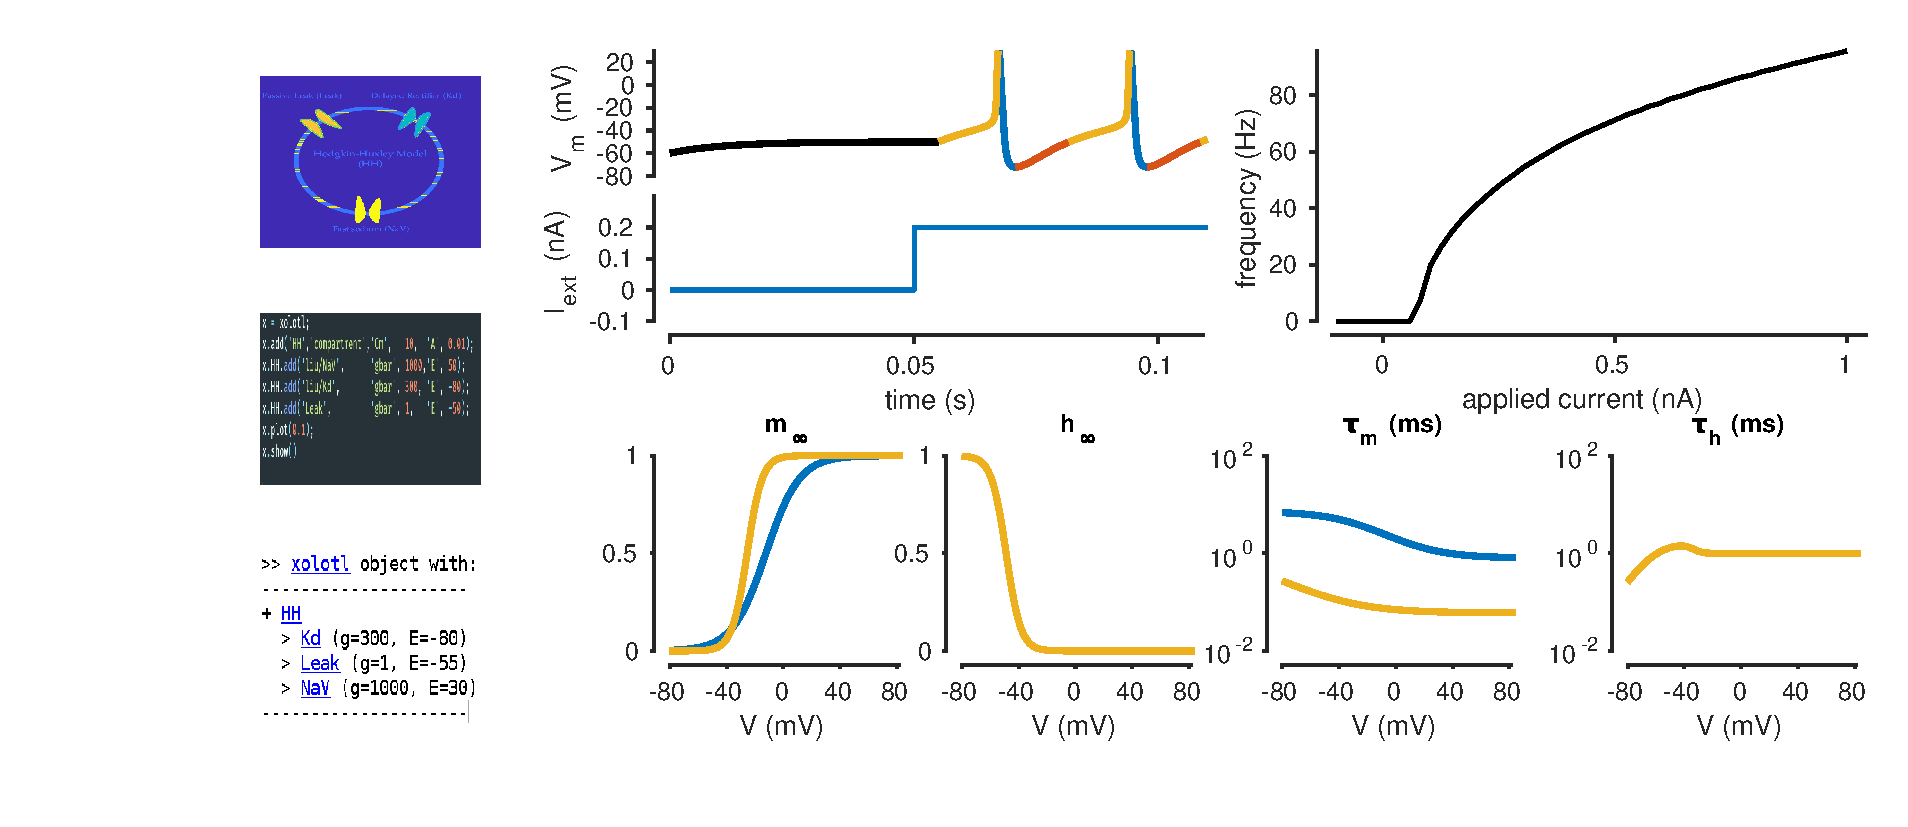
\includegraphics[width=1.0\linewidth]{gfx/figure_HH}
	\caption{\texttt{xolotl} can quickly set up and simulate conductance-based models. (A) Cartoon of a Hodgkin-Huxley single-compartment neuron model with fast sodium, delayed rectifier, and leak currents. (B) Code snippet in \texttt{MATLAB} used to implement D, F-I. (C) \texttt{xolotl} schematic displayed in the \texttt{MATLAB} command prompt. (D) Simulated voltage trace of a Hodgkin-Huxley model with three conductances and 0.2 nA of injected current. Colors indicate the dominant current (gold is fast sodium, blue is delayed rectifier, red is leak). (E) Firing rate-input relation displaying firing rate as a function of injected current current. (F-G) Steady-state gating functions for activation (m) and inactivation (h) gating variables. (H-I) Voltage-dependence of time constants for activation (m) and inactivation (h) gating variables. Variables not plotted are unity for all voltage.}
	\label{fig:figurehh}
\end{figure}

\begin{figure}
	\centering
	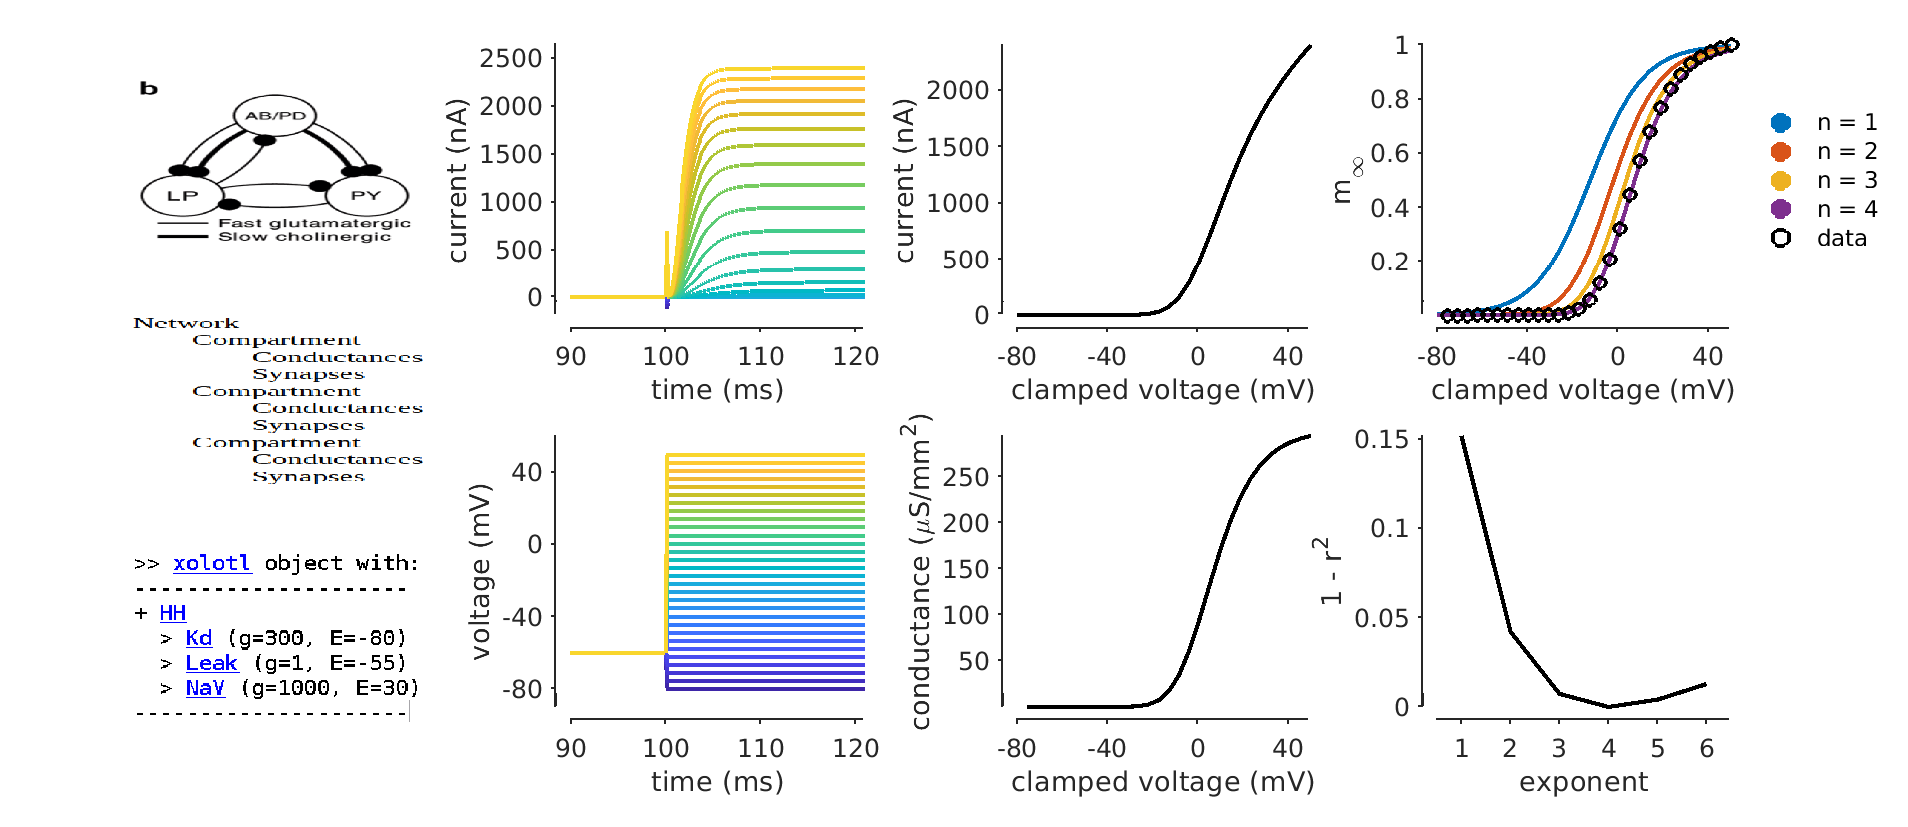
\includegraphics[width=1.0\linewidth]{gfx/figure_clamp}
	\caption{Simulating a voltage-clamp experiment. (A) Cartoon of a cell with delayed rectifier potassium conductance \autocite{liuModelNeuronActivitydependent1998} with experimentally-fixed voltage. (B) Structure of \texttt{xolotl} object in A. (C) Code snippet depicting integration under voltage clamp. (D-E) Current response to steps in voltage from a holding potential of $V_m = -60$ mV. (F) Current-voltage relation of the steady-state current ($t = 400$ ms) indicating a reversal potential of $E = -80$ mV and no inactivation. (G) Conductance-voltage relation at steady-state takes the form of a sigmoid. (H) Sigmoids $m$ fit to the model as $m^n$ data indicating that $n=4$ is the best fit. (I) Goodness of fit vs. exponent $n$, suggesting $n=4$ as the best fit to the data.}
	\label{fig:figureclamp}
\end{figure}

\begin{figure}
	\centering
	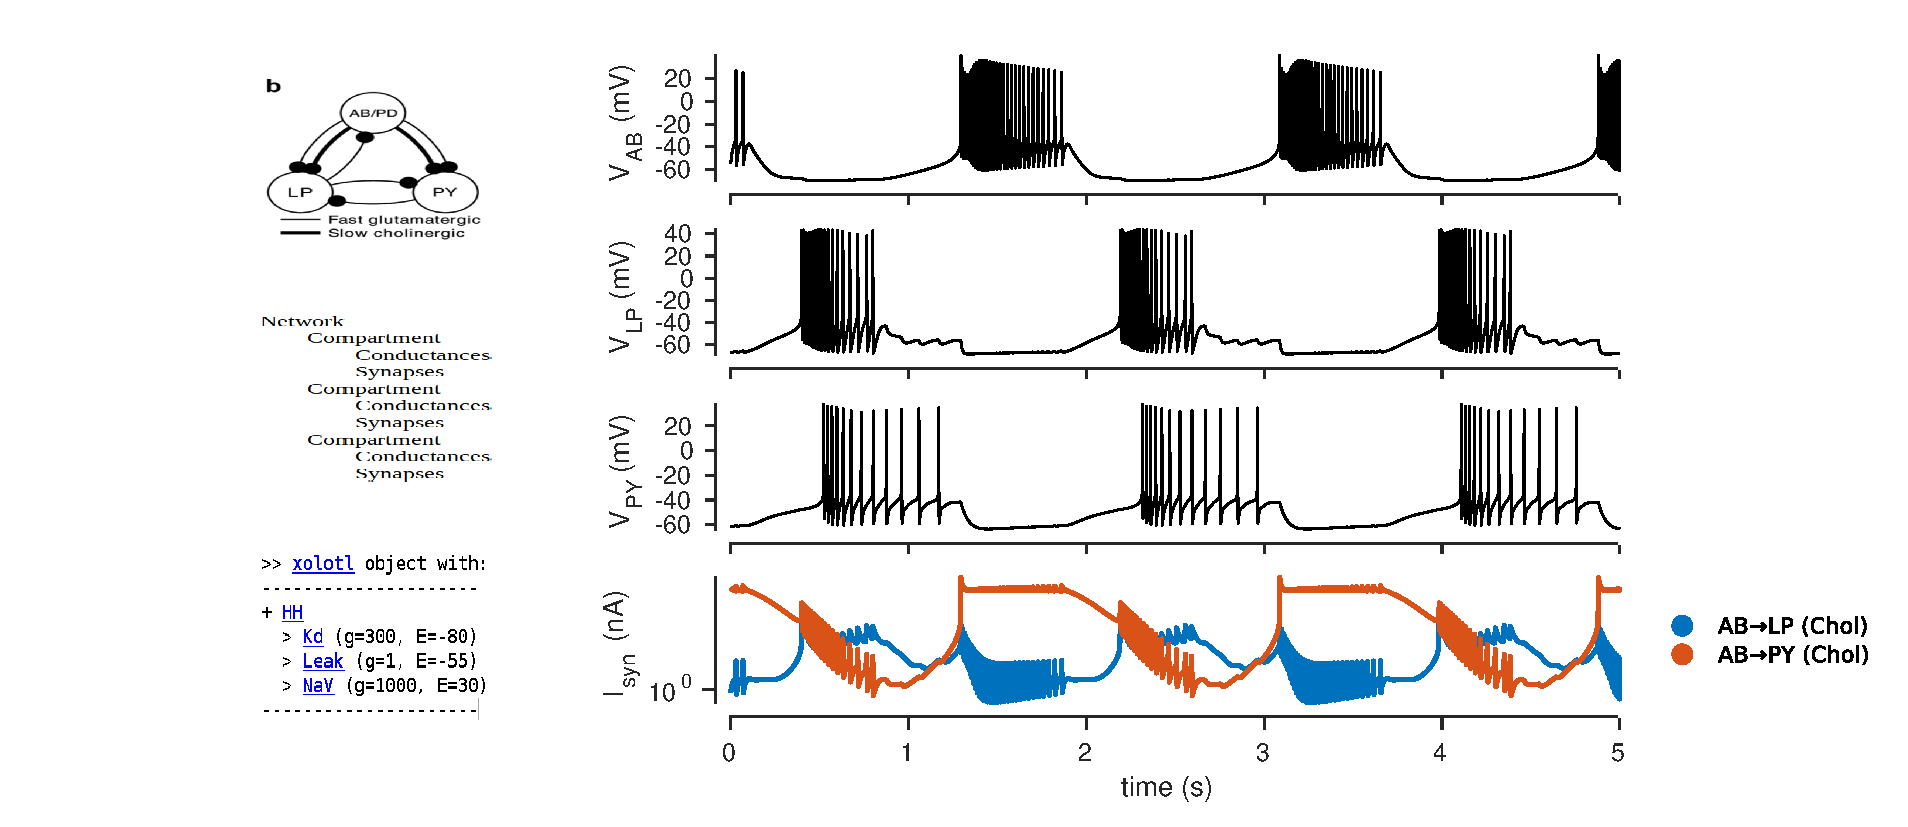
\includegraphics[width=1.0\linewidth]{gfx/figure_network}
	\caption{Simulating a network of conductance-based model neurons. (A) Diagram of a network model of the pyloric rhythm in the crustacean stomatogastric ganglion (Prinz \textit{et al.} 2004). (B) Each neuron is modeled as a single compartment with 7-8 intrinsic conductances and 1-3 post-synaptic conductances. (C) \textit{xolotl} implements conductances as fields of compartments and synapses as connections between compartments. (D-F) Simulated voltage trace of a model network for the three compartments. (G) Time series of synaptic currents in the simulated network can be obtained from the integration.}
	\label{fig:figurenetwork}
\end{figure}

\begin{figure}
	\centering
	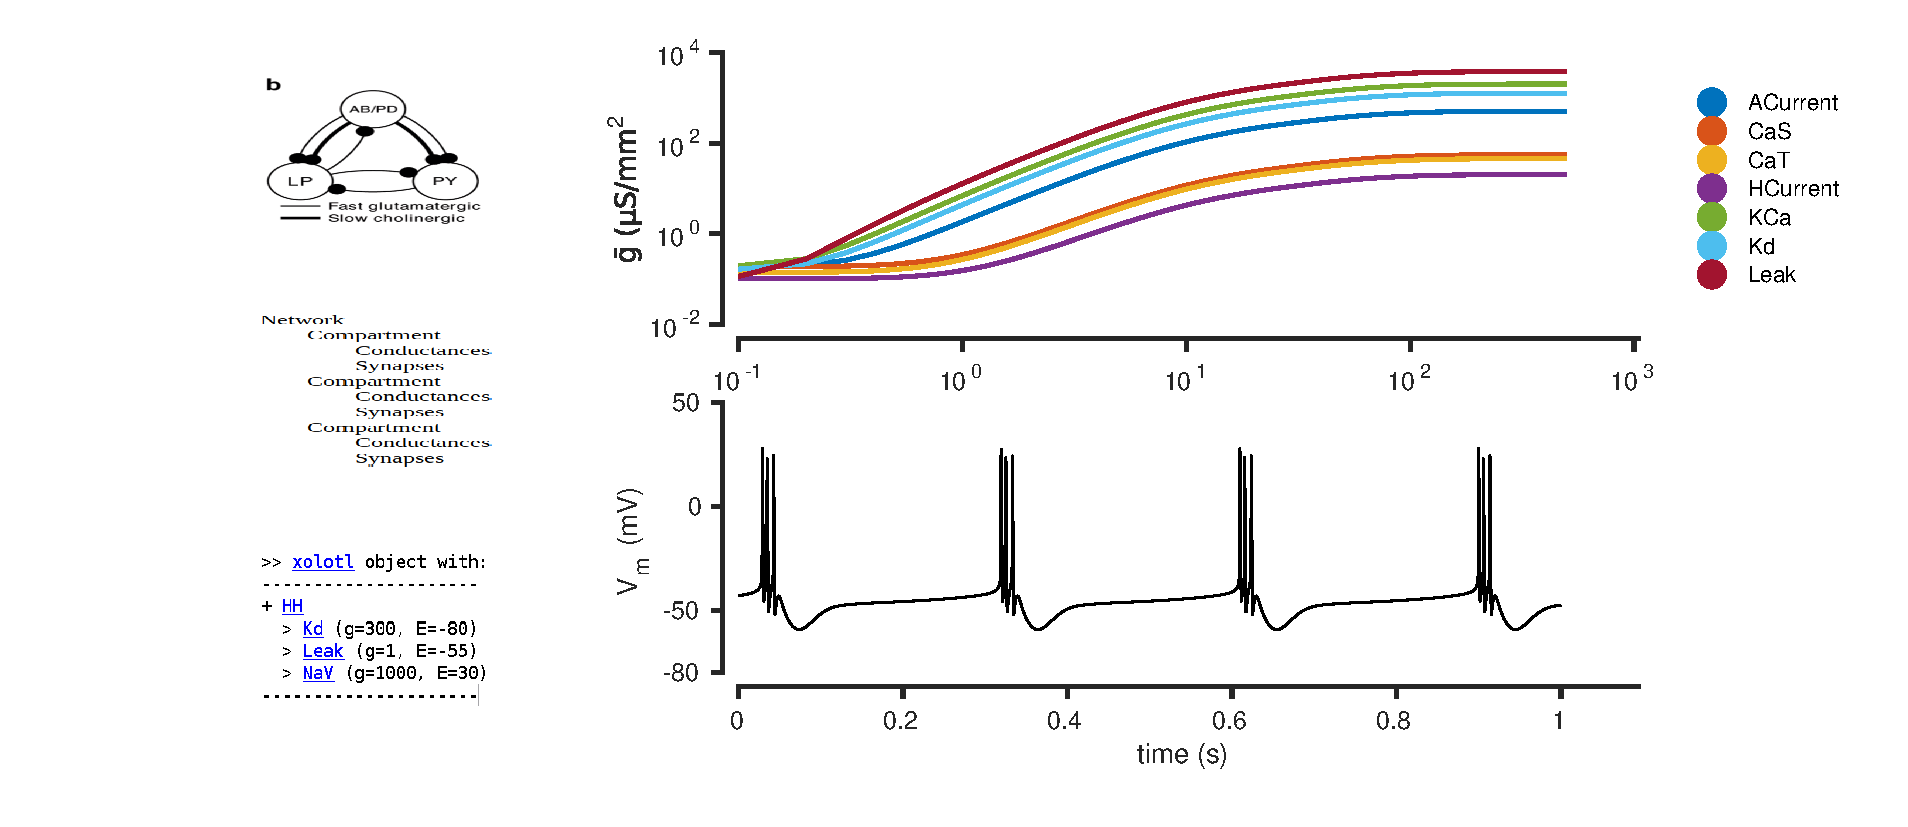
\includegraphics[width=1.0\linewidth]{gfx/figure_integral_control}
	\caption{Simulating neurons under homeostatic regulation. (A) Cartoon of a model neuron \autocite{liuModelNeuronActivitydependent1998} with integral control \autocite{olearyCorrelationsIonChannel2013}. (B) Hierarchical structure of a neuronal network considers controllers as components of compartments which act on conductances. (C) \texttt{xolotl} implements controllers XYZ. (D) Calcium sensors change maximal conductances to move a neuron from quiescence to a bursting state. (E) Voltage trace shows regular bursting activity after integral control.}
	\label{fig:figureintegralcontrol}
\end{figure}

\begin{figure}
	\centering
	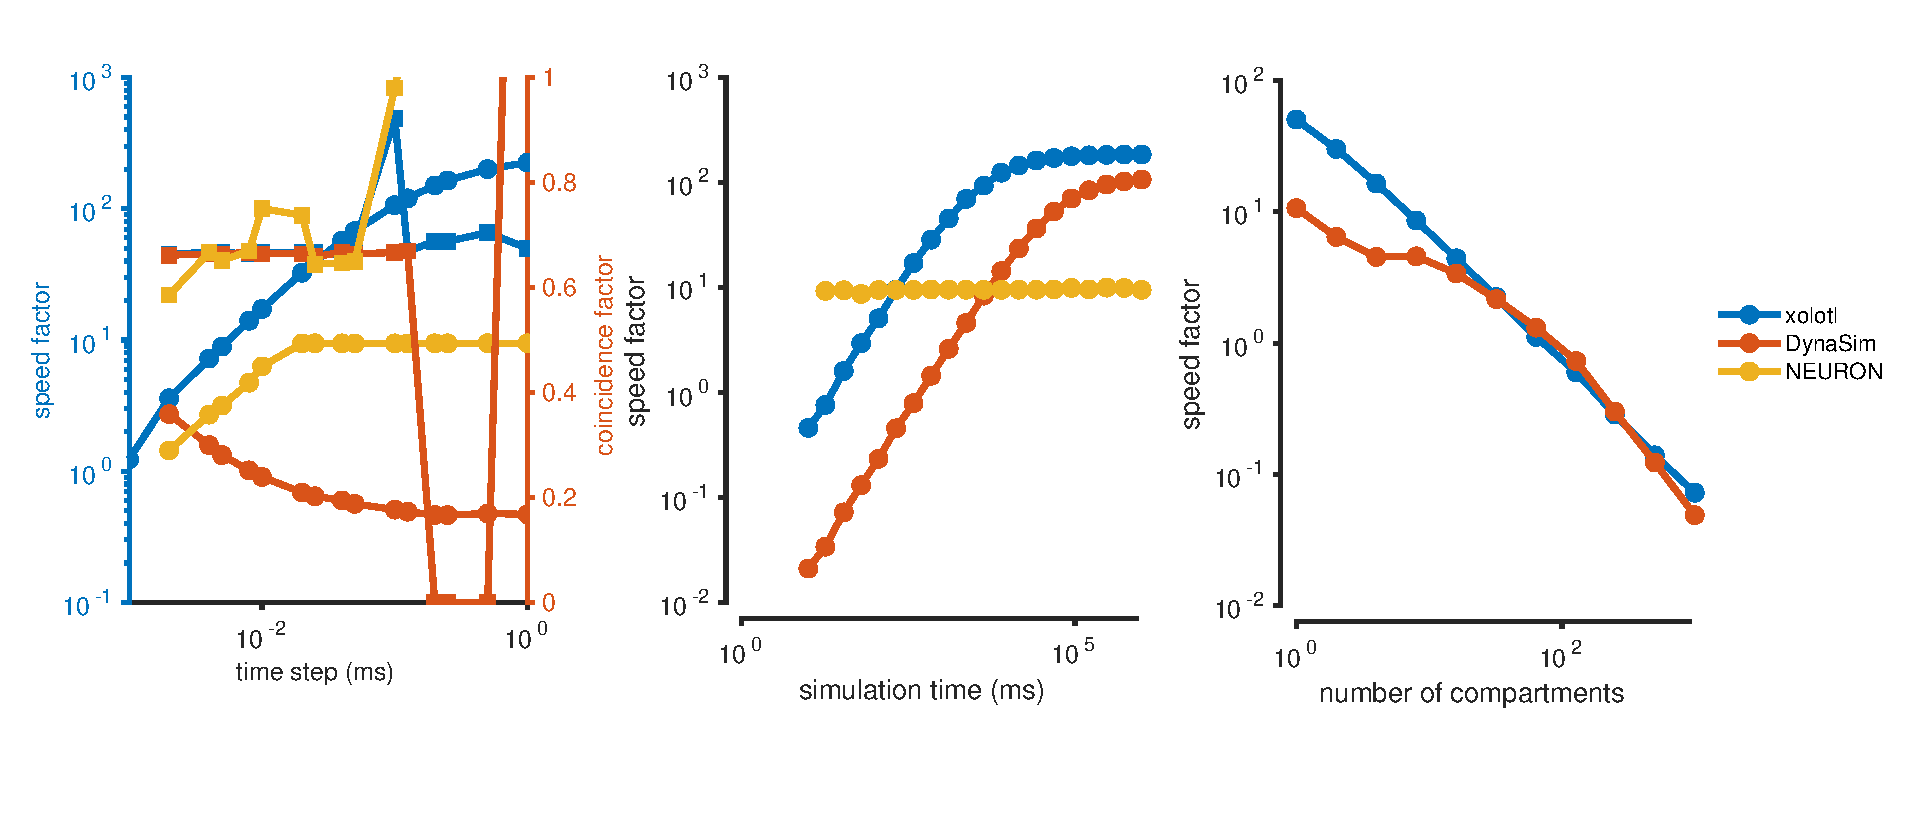
\includegraphics[width=1.0\linewidth]{gfx/figure_benchmark}
	\caption{\texttt{xolotl} benchmarked against \texttt{DynaSim}.}
	\label{fig:figurebenchmark}
\end{figure}


\end{document}
